% #############################################################################
% This is Chapter 5
% !TEX root = ../main.tex
% #############################################################################
% Change the Name of the Chapter i the following line
\fancychapter{Forecasting Model Selection}
\cleardoublepage
% The following line allows to ref this chapter
\label{chap:implementation}

So far, we have introduced the topic of this thesis and the objective of the work developed in Chapter \ref{chap:intro}, we have also presented some studies developed in this area in Chapter \ref{chap:background}, we have presented the concrete case studied used in Chapter \ref{chap:architecture}, and we have introduced the models implemented in this thesis in Chapter\ref{chap:Model}.
In this chapter, we present the environment in which the proposed models were trained, the datasets and all the data cleaning and preparation procedure, and finally the metrics used to evaluate the performance of the proposed models.
 

\section{Implementation environment} \label{chap5:enviromnet}

During the development of the thesis, several scripts were implemented, both for data processing and for the implementation of machine learning models. The language chosen for this purpose was \textit{Pyhton}. The primary reasons for this choice were the ease of syntax of this language, as well as the large number of libraries available, including \textit{keras}, a Deep Learning library that provides all the necessary tools for building and deploying Neural Networks.

Regarding the hardware components used, two different systems were used during the development of this work. The first environment consists of a CPU (Intel Core i5-3470 3.20GHz), and a GPU (NVIDIA GeForce GTX 1050 Ti) essential to accelerate the training process of the proposed models. The second environment consists of a virtual environment implemented on \textit{Microsoft Azure Machine Learning} platform, where a cluster consisting of a 6 core processor, and a GPU (NVIDIA Tesla K80).

The first setup was used with the purpose of testing, in a first phase, several models with simple tasks, and the second environment was used to put into practice more complex tests that required more computational capacity.
	

\section{Dataset}\label{chap5:dataset}

In this section, we describe the datasets used in the development of this work, and also detail the data preprocessing applied to the datasets so that they had the necessary formatting to be used during this experiment.

\subsection{Data description}

In the day to day of a building, there are many factors that influence its consumption and consequently the available power. In Chapter \ref{chap:background} some examples of work developed with the objective of predicting the energy consumption of a building were mentioned. In Appendix B, Table \ref{table1}, it is possible to verify that generally, two categories of data are used in this kind of applications, data that concern the behavior of the building, and climatic data that characterize the environment in which the building is located.

With respect to data on the behaviour of the building, \ac{EDP} provided two different datasets that present information between January 25, 2020 and September 30, 2020, totalling roughly 8 months of data, with a granularity of 5 seconds. The first dataset includes historical data regarding the energy consumption of the building, and the second dataset includes historical data regarding the solar production generated by the \ac{PV} panels present in the upper part of the building. It is also relevant to mention that the production data provided showed some gaps resulting from sensor reading failures. This aspect implies the need for some mechanisms to complete the missing data, which are described below.

Regarding climate data, \ac{FCUL} provided two different datasets that present information between January 25, 2020 and June 15, 2020, totaling more or less 5 months of data, with a granularity of 1 minute. The first dataset includes meteorological data regarding the geographical location of the building, and the second includes data regarding solar radiation exerted on the geographical area of the building. Neither of the two datasets had flaws.

In Table \ref{table2}, there is a summary of some key factors regarding the available datasets.


\begin{longtable}{|l|c|c|c|c|}
    \caption{Summary of the datasets used.}
    \label{table2}\\
    
    \hline & \multicolumn{2}{c|}{}&\multicolumn{2}{c|}{}\\[-0.5ex]
    \textbf{Dataset Provider}   & \multicolumn{2}{c|}{\textbf{EDP}} & \multicolumn{2}{c|}{\textbf{FCUL}}\\[1ex]
    \hline & \multicolumn{2}{c|}{}&\multicolumn{2}{c|}{}\\[-0.5ex]

    
    \textbf{Dataset} & \multicolumn{1}{l|}{\textbf{Consumption}} & \textbf{Production} & \multicolumn{1}{l|}{\textbf{Meteorological}} & \textbf{Radiation}  \\
    \textbf{Nº of variables} & \multicolumn{1}{c|}{8} & \multicolumn{1}{c|}{7} &  22  & \multicolumn{1}{c|}{28} \\
    \textbf{Preiod} & \multicolumn{2}{c|}{8 months and 5 days} & \multicolumn{2}{c|}{4 months and 21 days}  \\
    \multicolumn{1}{|r|}{Begin} & \multicolumn{2}{c|}{25-01-2020} & \multicolumn{2}{c|}{25-01-2020} \\
    \multicolumn{1}{|r|}{End}  & \multicolumn{2}{c|}{30-09-2020}  & \multicolumn{2}{c|}{15-06-2020} \\
    \textbf{Nº of days}       & \multicolumn{2}{c|}{249}     & \multicolumn{2}{c|}{142}    \\             
    \textbf{Nº of samples}    & \multicolumn{2}{c|}{4302720} & \multicolumn{2}{c|}{2453760} \\[1ex]
    \hline
    

\end{longtable}

As can be seen through the analysis of Table \ref{table2}, the data provided do not portray the same time window nor have the same granularity. It is then necessary to proceed to some data treatment in order to obtain the data in the desired form.

\subsection{Data manipulation}\label{sec:data_manip}

The data manipulation consists of a process in which the data made available is formatted in such a way that it meets the essential criteria to enable its introduction in the models. During the development of the thesis, this was the most time consuming process. The data treatment is an extremely demanding process, which is simplified in the diagram of Figure \ref{datatreatment}.

\begin{figure}[h!]
    \centering
    \begin{center}
    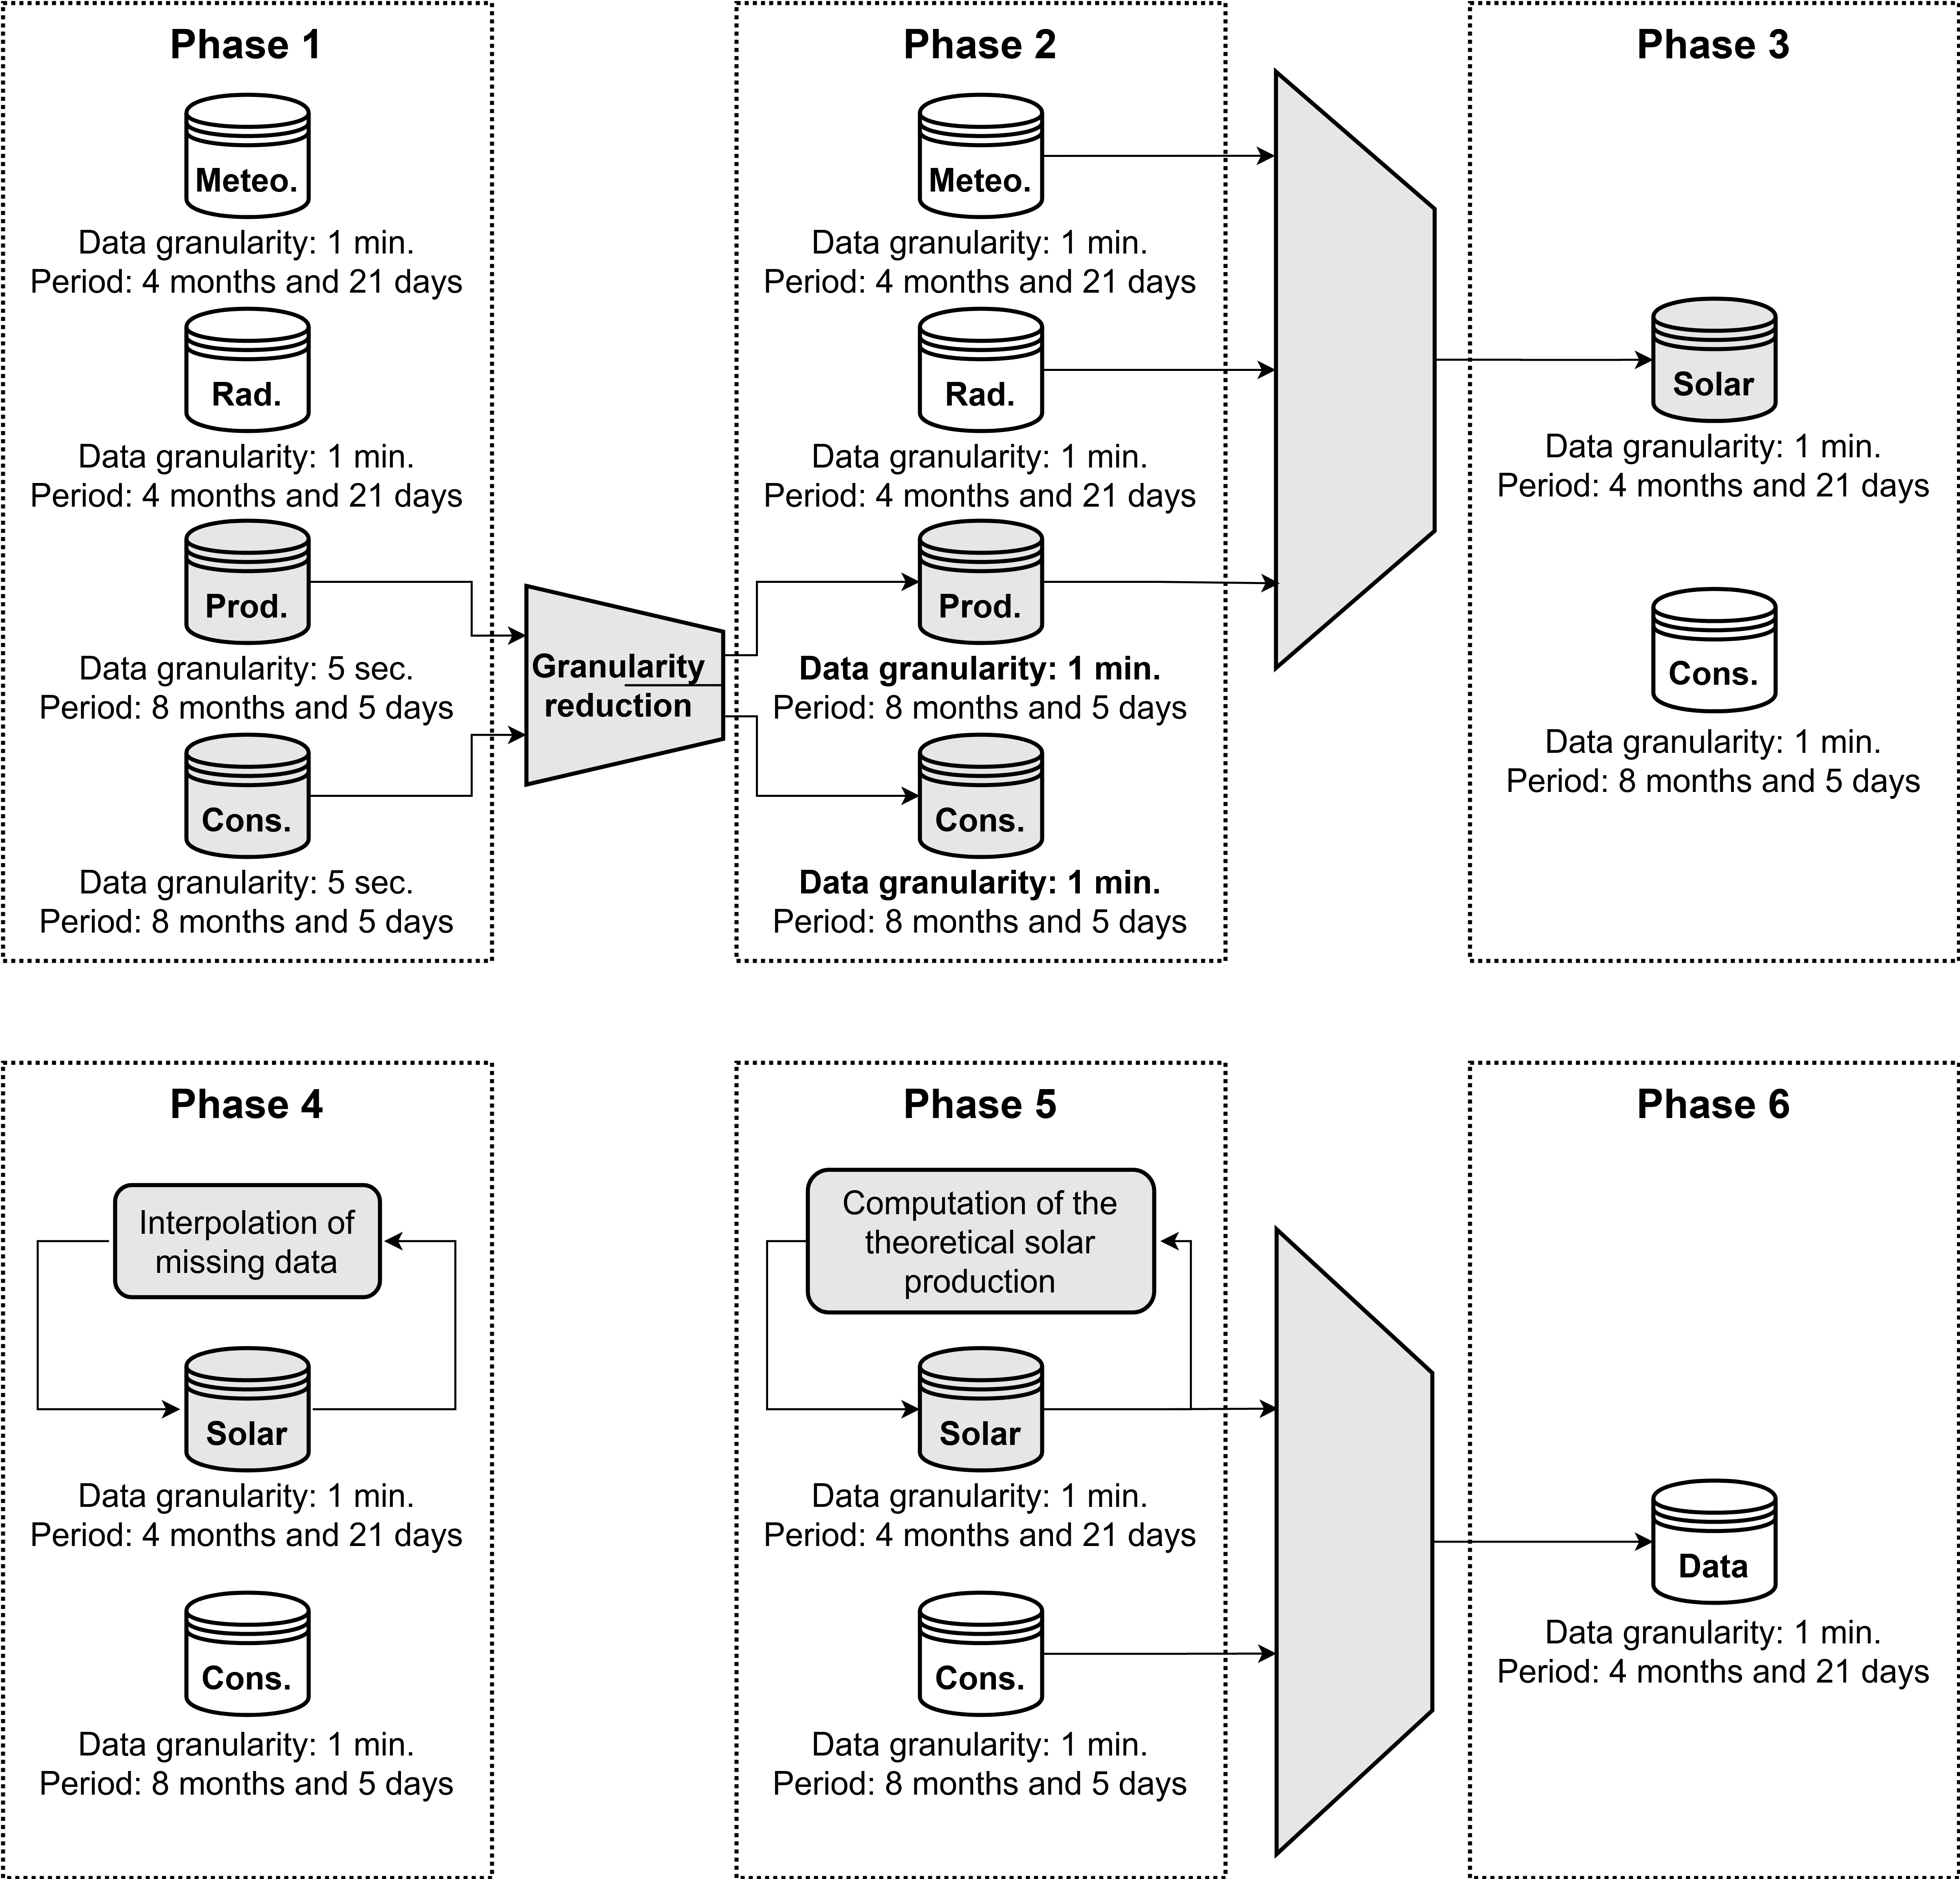
\includegraphics[width=1\textwidth]{Images/Data.png}
    \caption{Data treatment process.}
    \label{datatreatment}
    \end{center}
\end{figure}

In Phase 1, the production data (Prod.) is incomplete due to failure of the system responsible for acquiring and storing this indicator. There is also a difference both in granularity and period available, between the data provided by \ac{EDP} and the data provided by \ac{FCUL}. It is then necessary, first of all, to equal the granularity of all four datasets. In order to do that, a function was applied to reduce the granularity of the production (Prod.) and consumption (Cons.) datasets, forcing the frequency of both datasets to one minute. the  The function applies an arithmetic mean given by 

\begin{equation}
     A={\frac {1}{n}}\sum _{i=1}^{n}a_{i}={\frac {a_{1}+a_{2}+\cdots +a_{n}}{n}},
\label{amean}
\end{equation}

where $A$ represents the value of the final measure with frequency of 1 minute, and $n$ represents the number of nodes between that minute range that will be converted to a single value. We then reached Phase 2, where the four datasets have the same granularity. Then, the datasets corresponding to the meteorological data (Meteo.), radiation data (Rad.) and production data (Prod.) are concatenated. As a result of this process (Phase 3), the dataset (Solar) is formed, which aggregates all the information regarding climate data and solar production data over a period of 4 months and 21 days. The reason behind this phenomenon is that all the production days for which there is no direct correspondence in the meteorological data (Meteo.) and radiation data (Rad.) datasets are dropped. 

As mentioned before, the data regarding the solar production (Prod.) presented some temporal flaws. In order to solve the problem, two solutions were found. For time gaps of less than 30 minutes (Phase 4), a quadratic interpolation was applied. As an example, given any three points $(x_0, f(x_0))$, $(x_1, f(x_1))$ and $(x_2, f(x_2))$, the polynomial that interpolates the three points is given by

\begin{equation}
\begin{split}
     & f_2(x)=b_0+b1(x-x_0)+b_2(x-x_0)(x-x1),\\
     & where:\\
     & b_0=f(x_0),\\
     & b_1=f[x_0,x_1]=\frac{f(x_1)-f(x_0)}{x_1-x_0},\\
     & b_2=f[x_0,x_1,x_2]=\frac{\frac{f(x_2)-f(x_1)}{x_2-x_1}-\frac{f(x_1)-f(x_0)}{x_1-x_0}}{x_2-x_0}.\\
\end{split}
\label{poly}
\end{equation}

In order to exemplify the evolution of the incomplete dataset construction, in the graph of Figure \ref{int0} we can observe the solar power generated measured by the sensors on February 3, 2020. In red, is the portion of data that were measured, corresponding to the Solar dataset in Phase 3 represented in Figure \ref{datatreatment}. After the interpolation, to the original dataset are added the points represented in blue, which represent measurement failures of less than 30 minutes. At the end of Phase 4, the dataset is then composed of the data points represented in blue plus the points represented in red.



\begin{figure}[h!]
    \centering
    \begin{center}
    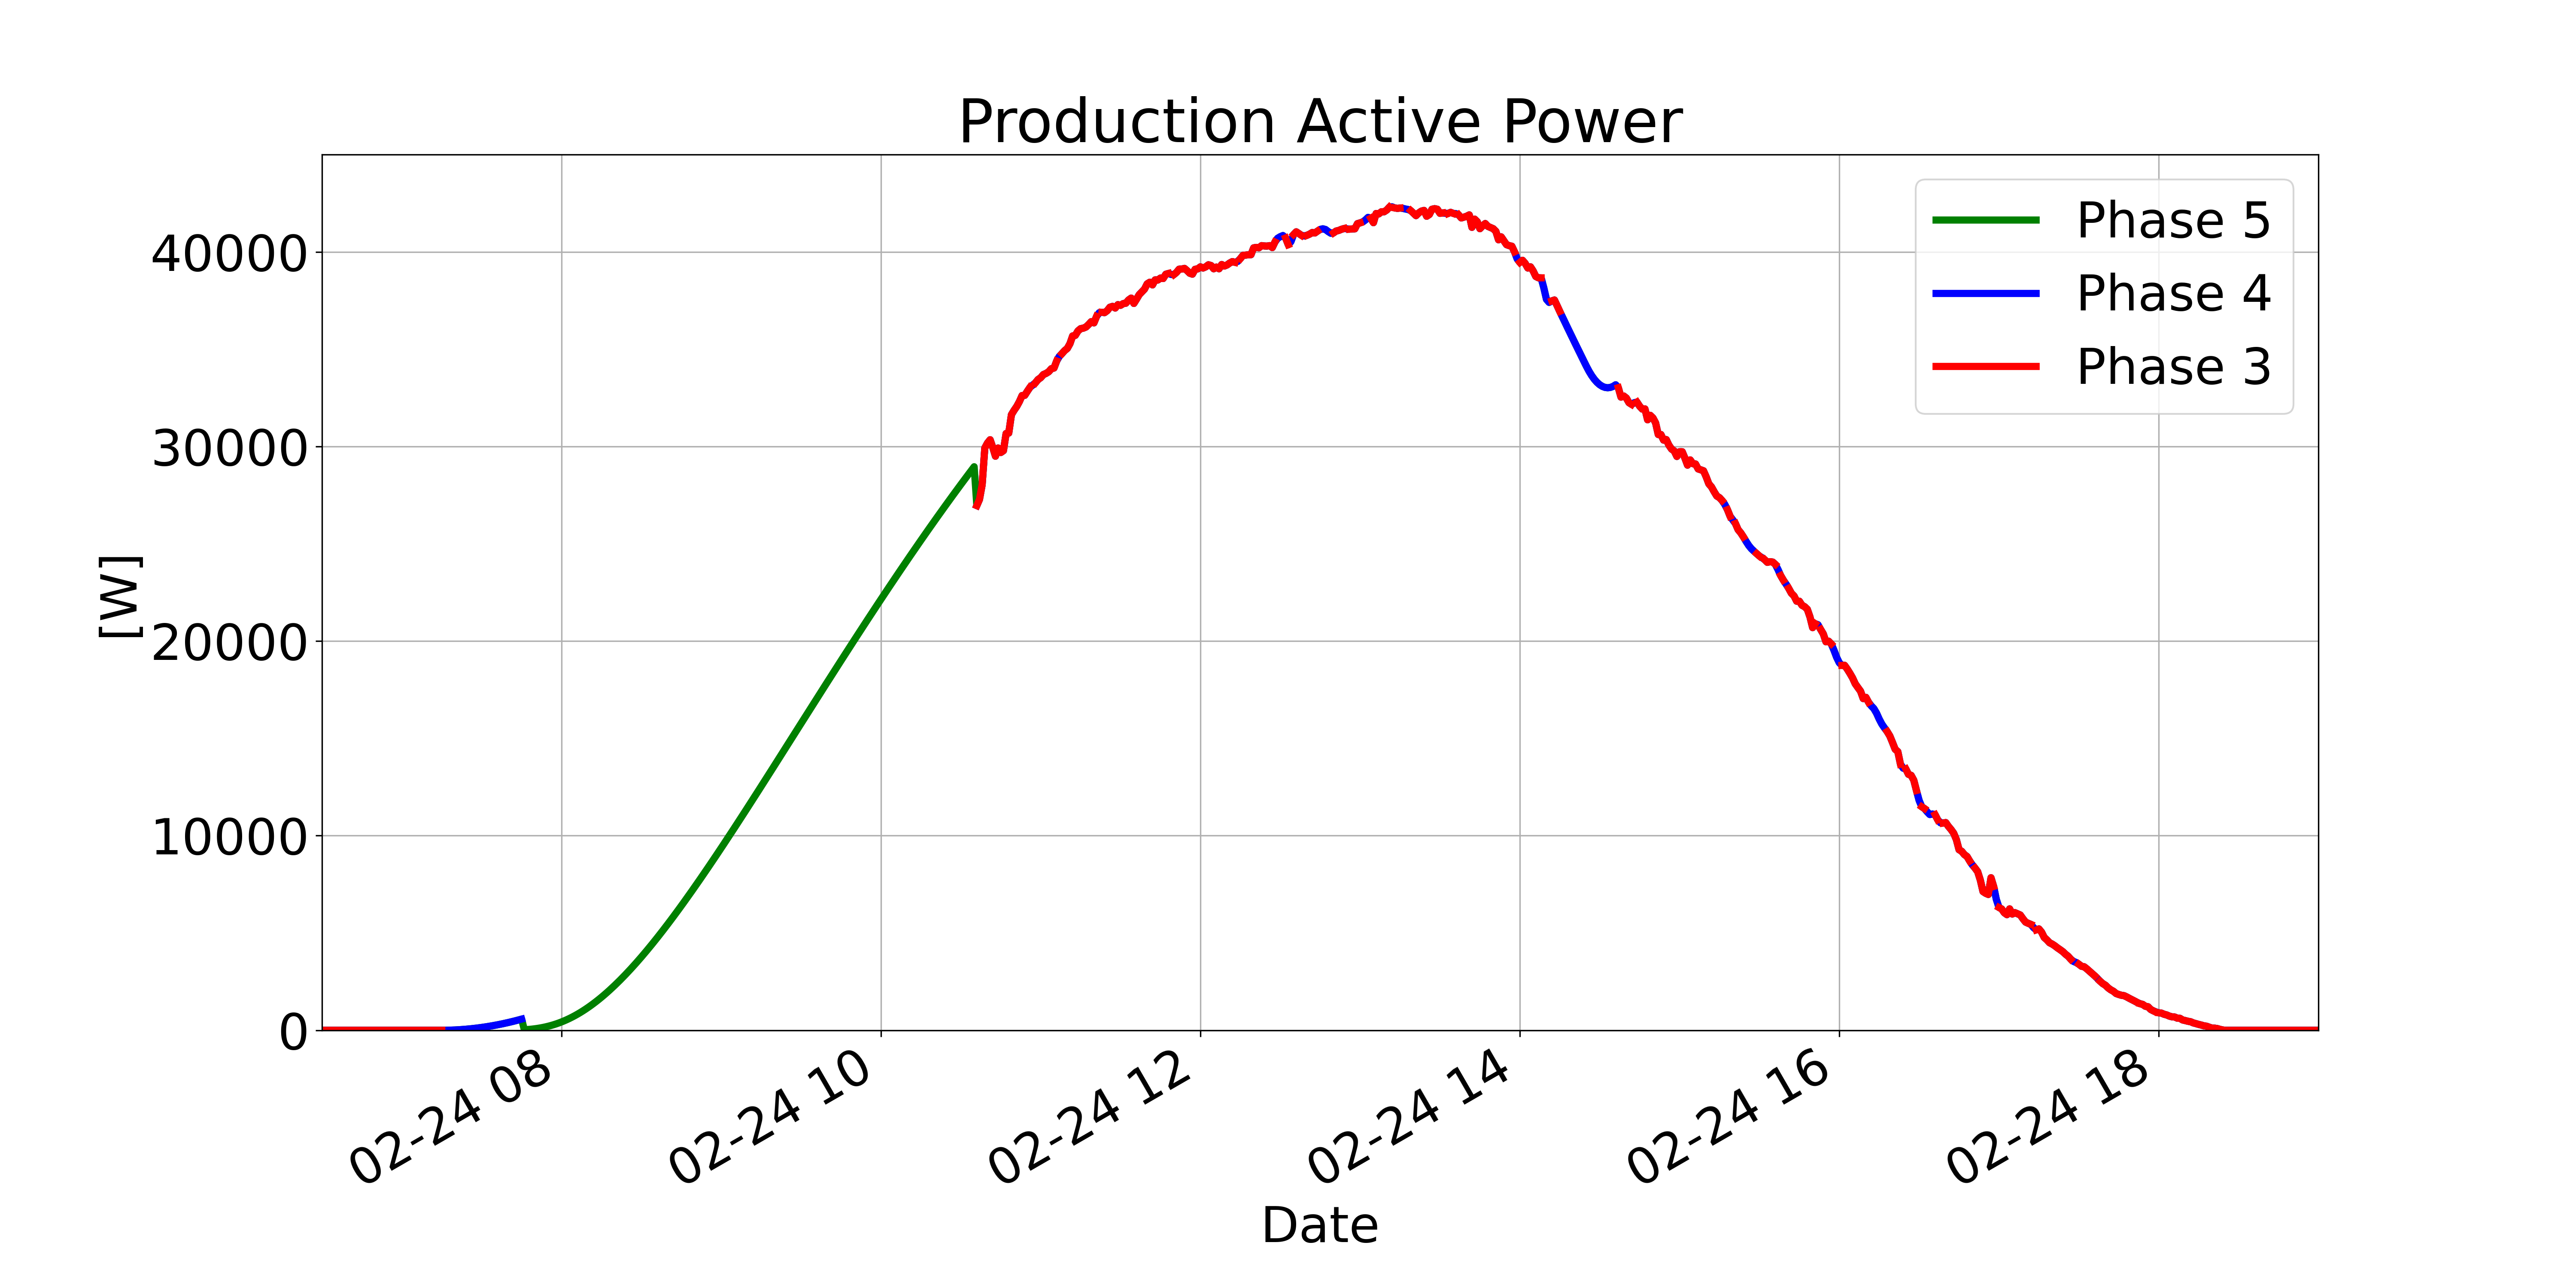
\includegraphics[width=1\textwidth]{Images/int0.png}
    \caption{Data treatment process.}
    \label{int0}
    \end{center}
\end{figure}





For time failures of more than 30 minutes, the dataset was completed with theoretically computed values, since the interpolation for large temporal failures does not present the expected behavior.
Based on the equation of the sun's position in the sky throughout the year, the maximum amount of solar insolation on a surface at a particular tilt angle can be calculated as a function of latitude and day of the year\cite{solar0}. In order to determine the direct component of solar radiation in $kW/m^2$, we used


\begin{equation}
     I_D = I_0*0.7^{(AM^{0.678})}
\label{solar}
\end{equation}

where $I_0$ is the solar intensity external to the Earth's atmosphere that is approximately $1.353 kW/m^2$, $0.7$ represents the overall attenuation of the atmosphere, $AM = \frac{1}{cos\theta}$ is the airmass and $\theta$ is the zenith angle (90° minus the altitude) of the sun. This formula produces an optimal result when there are no clouds. Multiplying the resulting value by the total area of panels in the building and taking into account their positioning efficiency, a theoretical value of power generated by the \ac{PV} panels is obtained, in an ideal scenario. In Phase 5, all missing readings were replaced by the calculated theoretical value, as can be seen in Figure \ref{int0} in green. This way, the Solar dataset was completed. It is possible to verify that the point of change between the theoretical data (the green one) and the original data (the red one) is somewhat sudden, because the green signal considers an ideal scenario and the red signal represents real measurements (affected by clouds, cranes, etc.) The sum of the green, blue and red signals, result in a complete signal for the solar active power generated by the \ac{PV} panels.


In Phase 6 the Solar and Cons. datasets were concatenated, thus reducing the dataset time interval to a final result of 4 months and 21 days.


\subsection{Feature selection}

Although a huge amount of data was made available for the development of this study, the use of a large number of different features may negatively affect the performance of the tested models, namely their speed. In order not to overload the models, an initial set of features from all the available datasets was selected. In Table \ref{table3} the reader may find the selected features, their unit and their descrption.



\begin{table}[htbp]
  \centering
  \caption{Features used.}
    \begin{tabular}{rlcl}
    \toprule
          & \multicolumn{1}{c}{\textbf{Feature}} & \textbf{Unit} & \multicolumn{1}{c}{\textbf{Description}} \\
    \midrule
    Input & Std\_DHI & W/$m^2$ & Standard diffuse horizontal irradiance \\
          & Avg\_DHI & W/$m^2$ & Average diffuse horizontal irradiance \\
          & Avg\_GHI & W/$m^2$ & Global horizontal irradiance \\
          & Avg\_DNI & W/$m^2$ & Direct normal irradiance \\
          & Avg\_POA & W/$m^2$ & Average plane of array \\
          & T\_amb\_avg & C     & Average ambient temperature \\
          & TheoreticalValue & W     & Theoretical production active power generated \\
          & ActPwr & W     & Production active power \\
          & Ir    & A     & Consumption three-phase current \\
          & Is    & A     & Consumption three-phase current \\
          & It    & A     & Consumption three-phase current \\
          & Vrs   & V     & Consumption three-phase voltage \\
          & Vst   & V     & Consumption three-phase voltage \\
          & Vtr   & V     & Consumption three-phase voltage \\
          & P     & W     & Consumption real power \\
          & S     & VA    & Consumption complex power \\
          & hour  & hours & Hour of the day \\
          & day\_of\_moth & days  & Day of the month \\
          & day\_of\_week & days  & Day of the week \\
          & month & months & Month of the year \\
          & holiday & binary & National holiday identifier \\
          & Available Power & W     & Current available power \\
    \midrule
    Output & Available Power (t+5) & W     & Real available power for 5 minutes ahead \\
          & Available Power (t+10) & W     & Real available power for 10 minutes ahead \\
          & Available Power (t+15) & W     & Real available power for 15 minutes ahead \\
    \end{tabular}%
  \label{table3}%
\end{table}%






Although all these features contribute in some way to enrich the past information available, it is important to reduce as much as possible the number of features used as input to the model, limiting the choice to the essentials.
In this sense, a second phase of analysis was then carried out where the correlation matrix between each of the features was projected. In Figure \ref{corr} one can then observe the correlation matrix where the correlations between all the selected variables are represented. The value of the correlation is present in the [-1, 1] range, where -1 means that the variables present an opposite correlation, 0 means that there is no correlation between the two variables and 1 means that there is perfect correlation between the two variables. 


\begin{figure}[h!]
    \centering
    \begin{center}
    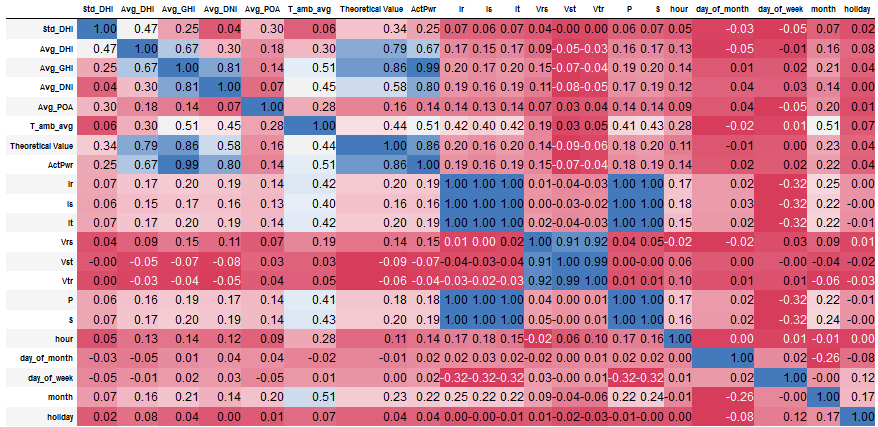
\includegraphics[width=1\textwidth]{Images/corr.PNG}
    \caption{Feature correlation matrix.}
    \label{corr}
    \end{center}
\end{figure}


The aim of computing this matrix is to identify variables that present a perfect or almost perfect correlation between them, in order to eliminate redundancies. 

A perfect correlation between two variables means that one can be deduced from the other, that is, the relevance of the two variables for the construction of the forecasting system is the same, so one of the variables can be eliminated. 


First of all, it was decided to eliminate the features that contribute to the calculation of others. In this sense, both three-phase voltages and three-phase currents contribute to the calculation of S and P and present a perfect correlation between them. It was then chosen to eliminate the features: Ir, Is, It, Vrs, Vst, Vtr. Then, since in this case S does not have an imaginary component, S and P have the same value. The feature S was then also eliminated. Also, although TheoreticalValue and Avg\_GHI present a very high correlation with ActPwr (which is predictable given that the measured ActPwr these two variables were added, as explained in section \ref{chap4:vtp}), we chose to keep these two variables as input features since the correlation is not exactly perfect and can be decisive in certain cases in building a good predictive model. Therefore, the variables chosen for the input of all tested models are: Std\_DHI, Avg\_DHI, Avg\_GHI, Avg\_DNI, Avg\_POA, T\_amb\_avg, Theoretical\ Value, ActPwr, P, hour, day\_of\_month, day\_of\_week, month and holiday. In addition, the variable Available Power given in W has been added as an input feature, resulting in a total of 15 input features and 3 output (Available Power in 5, 10 and 15 minutes).


\subsection{Data shifting}

While designing a predictive model, the training process is critical so that the model can learn from the data supplied to it. In a time series problem, it would not make sense for the input data to be of the same instant as the output data. When one wants to determine a future value based on current conditions, one needs to train the model to use the input data of the current instant to predict the output data of a future instant. It is then necessary to apply a shift to the output data so that training the model builds a predictive logic. If this shift wasn't applied, one would be training the model to, based on the current instant data, determine the output data of the current instant, and that is not what is intended. As it is already known, one of the main objectives of this thesis is to forecast the available power of the building in 5, 10 and 15 minutes. To do that, it is then necessary that the model can perform 3 forecasts, one for each of these scenarios. Consequently, it is also necessary to apply 3 different shifts to the training data. In Figure \ref{shifting}, the reader can find a graphical representation of the performed procedure.


\begin{figure}[h!]
    \centering
    \begin{center}
    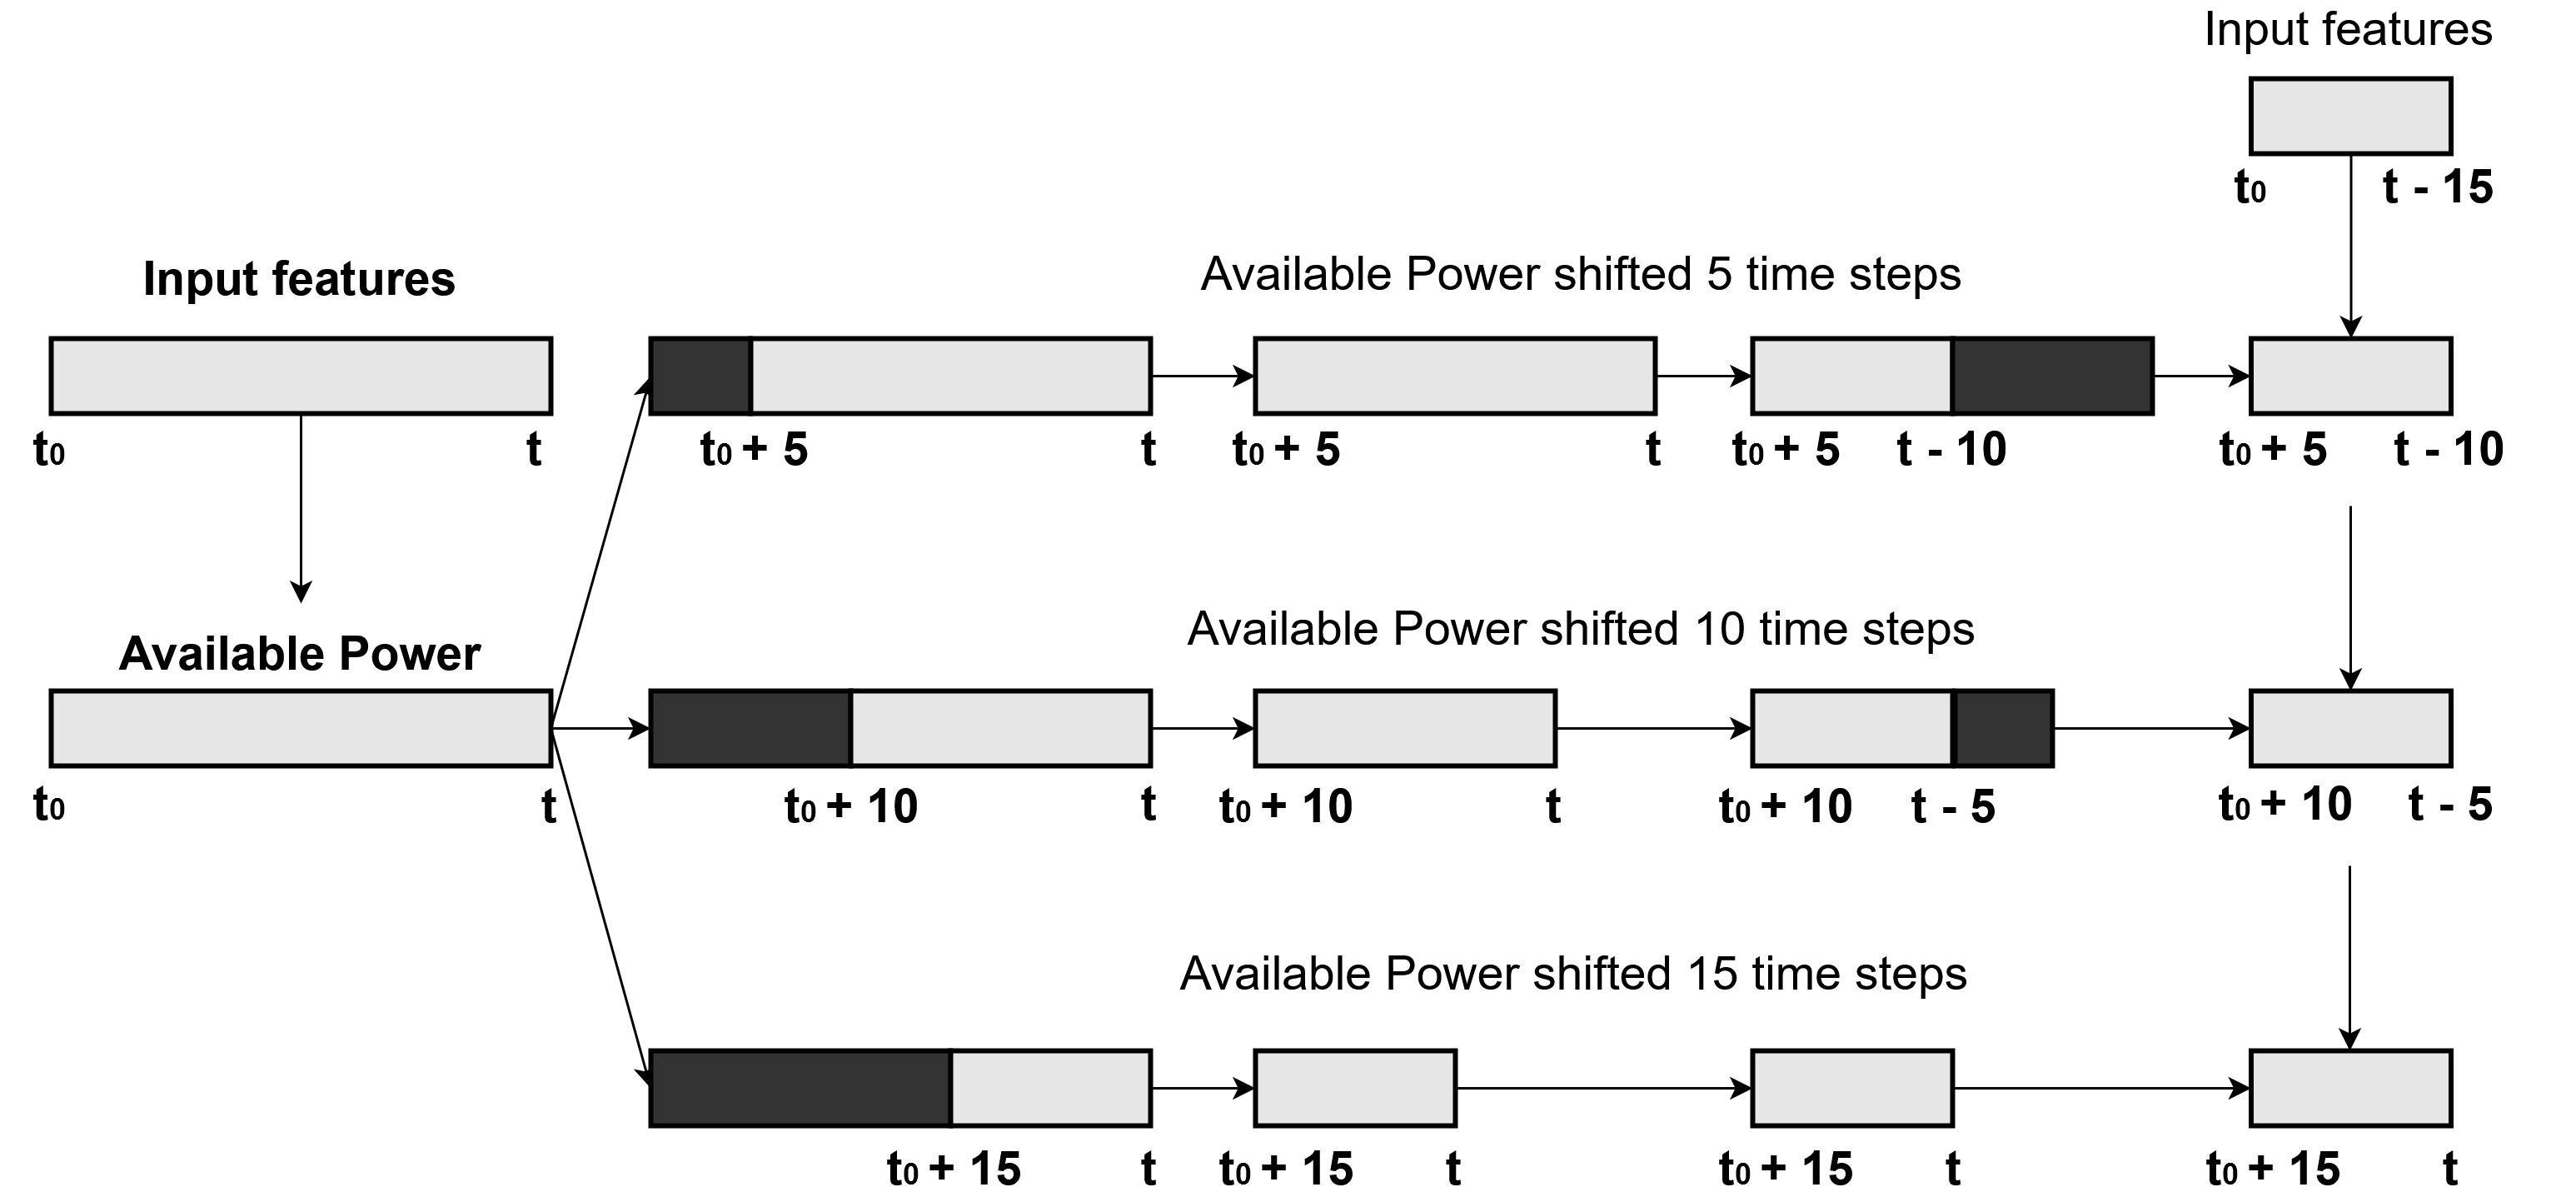
\includegraphics[width=1\textwidth]{Images/Data Shift.png}
    \caption{Data shifting procedure.}
    \label{shifting}
    \end{center}
\end{figure}

In a first instance one has the data set that corresponds to the 15 features identified in the previous section. For the initial scenario, the 15 features of a given instant $t_i$, have a direct match with a value of Available Power of the output variables for the same instant $t_i$.  Then the transformation process begins, where the output variables are shifted 5, 10 and 15 time-steps. The data vector of Available Power is copied originating three identical vectors. In the first step, the 5, 10 and 15 measurements of Available Power are removed originating the output vectors with the ranges $[t_0 + 5, t]$, $[t_0 + 10, t]$, $[t_0 + 15, t]$ respectively.  At this time each set of input features already presents a match of Available Power in 5, 10 and 15 minutes, but the output vectors present different dimensions as one would expect. In order to have output vectors with the same dimension, the size of the three vectors is limited to the size of the smallest, as well as the set of input features. In the last step there is then a set of input features with values in the range $[t_0, t-15]$ and the ranges $[t_0 + 5, t-10]$, $[t_0 + 10, t-5]$ and $[t_0 + 15, t]$ for the Available Power to 5, 10 and 15 minutes, all four vectors with the same dimension. It is now possible to train the model for the three proposed cases. It should be noted that although there is a reduction in the dataset dimension, this reduction is derisory for the data used. There is a loss of 15 time-steps of data in this whole process. Since the total dataset contains a total of 201542 time-steps, the elimination of these 15 time-steps corresponds to a loss of only 0.0074$\%$.

\subsection{Data partition}\label{sec:datap}

In order to study a certain algorithm, it is necessary to have access to past data to train the model and then evaluate its performance. The the available data is key point when it comes to developing predictive models. Usually, in \ac{ML}, to study a certain model, the dataset should be divided into three sets as can bee seen in Figure \ref{division}. 

\begin{figure}[h!]
    \centering
    \begin{center}
    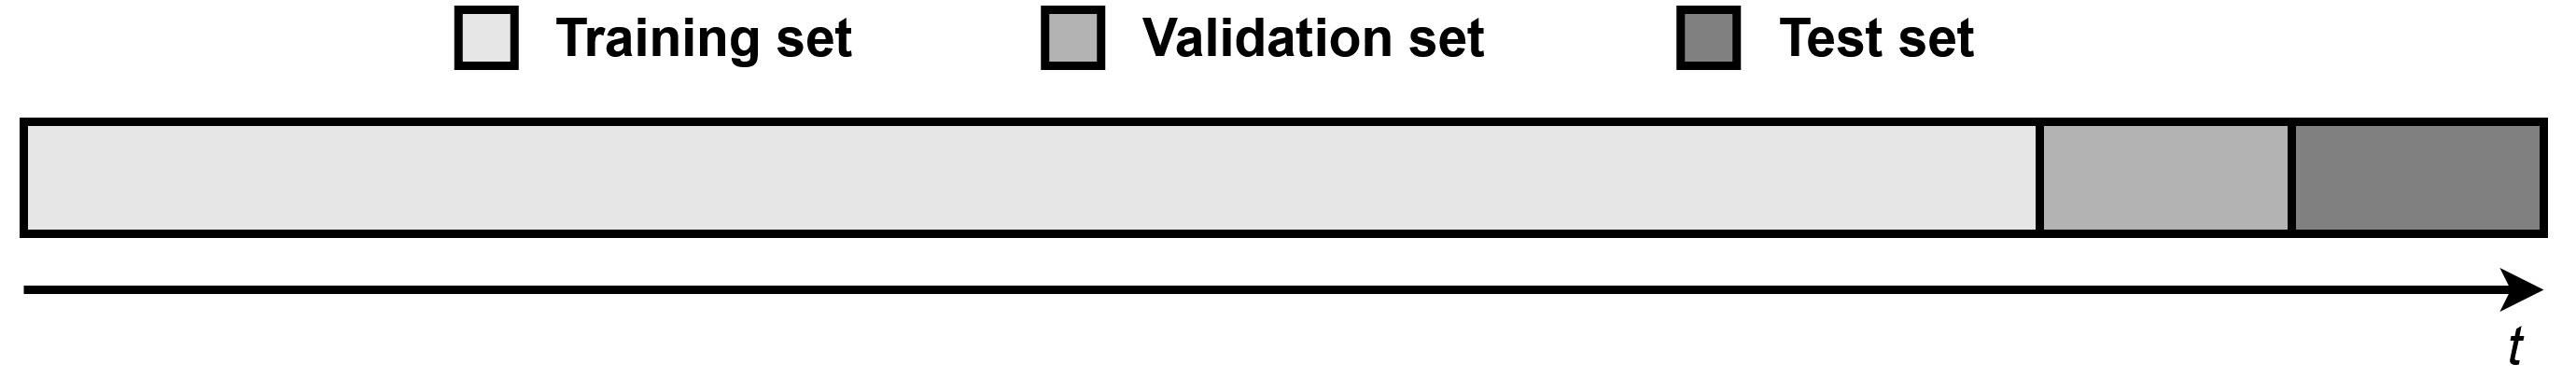
\includegraphics[width=1\textwidth]{Images/division.png}
    \caption{Dataset division.}
    \label{division}
    \end{center}
\end{figure}

The first set is known as a training set, and consists of a dataset used to feed the model with examples in order to fit the hyperparameters, such as the weights of connections between neurons in artificial neural networks. As the name implies, the training set is suitable to train the model, progressively adapting the model to its intended purpose. The second is the validation set, which is responsible for simultaneously continuing to adapt the hyperparameters of the model, while providing an unbiased evaluation of the model fit. In addition to that, it can be used for regularization, as is the case of eraly-stopping, referred to in section \ref{sec:early}. Finally, the test set is an independent dataset of the two previous ones, which has as main objective to evaluate in an unbiased way the performance of the model in unseen data (data that was not used neither in the training process nor in the validation process). 

One way to use the available dataset to evaluate the proposed models would be to simply apply the standard training-validation-testing division to the entire dataset available, but this strategy would be a poor way to use the small amount of data available. Typically, to evaluate machine learning models on a very limited time interval, k-fold cross-validation is used. However, cross-validation can present some problems when applied to time-series problems, since one cannot choose random samples and assign them to either the test set or the training set because it makes no sense to use future values to predict past values. There is a time dependency between observations, and it is essential to preserve this relationship during testing. To overcome this barrier, a block cross-validation method was used. This validation methodology consists, in the first place, of separating the training data into different blocks. Afterwards, each of these blocks must be used to train and validate the data. After applying this procedure to the different blocks, an average of the errors presented in the different blocks must then be calculated, thus reaching a total error value. 

In Figure \ref{partition} the reader may find six different sub-datasets, resulting from a division of the main datastet, defined in phase 6, of the section \ref{sec:data_manip}. The idea behind this division is, in a first stage, to use datasets 1, 2 and 3 for training and validation, in order to conduct hyperparameter tuning of the eight architectures proposed.

\begin{figure}[h!]
    \centering
    \begin{center}
    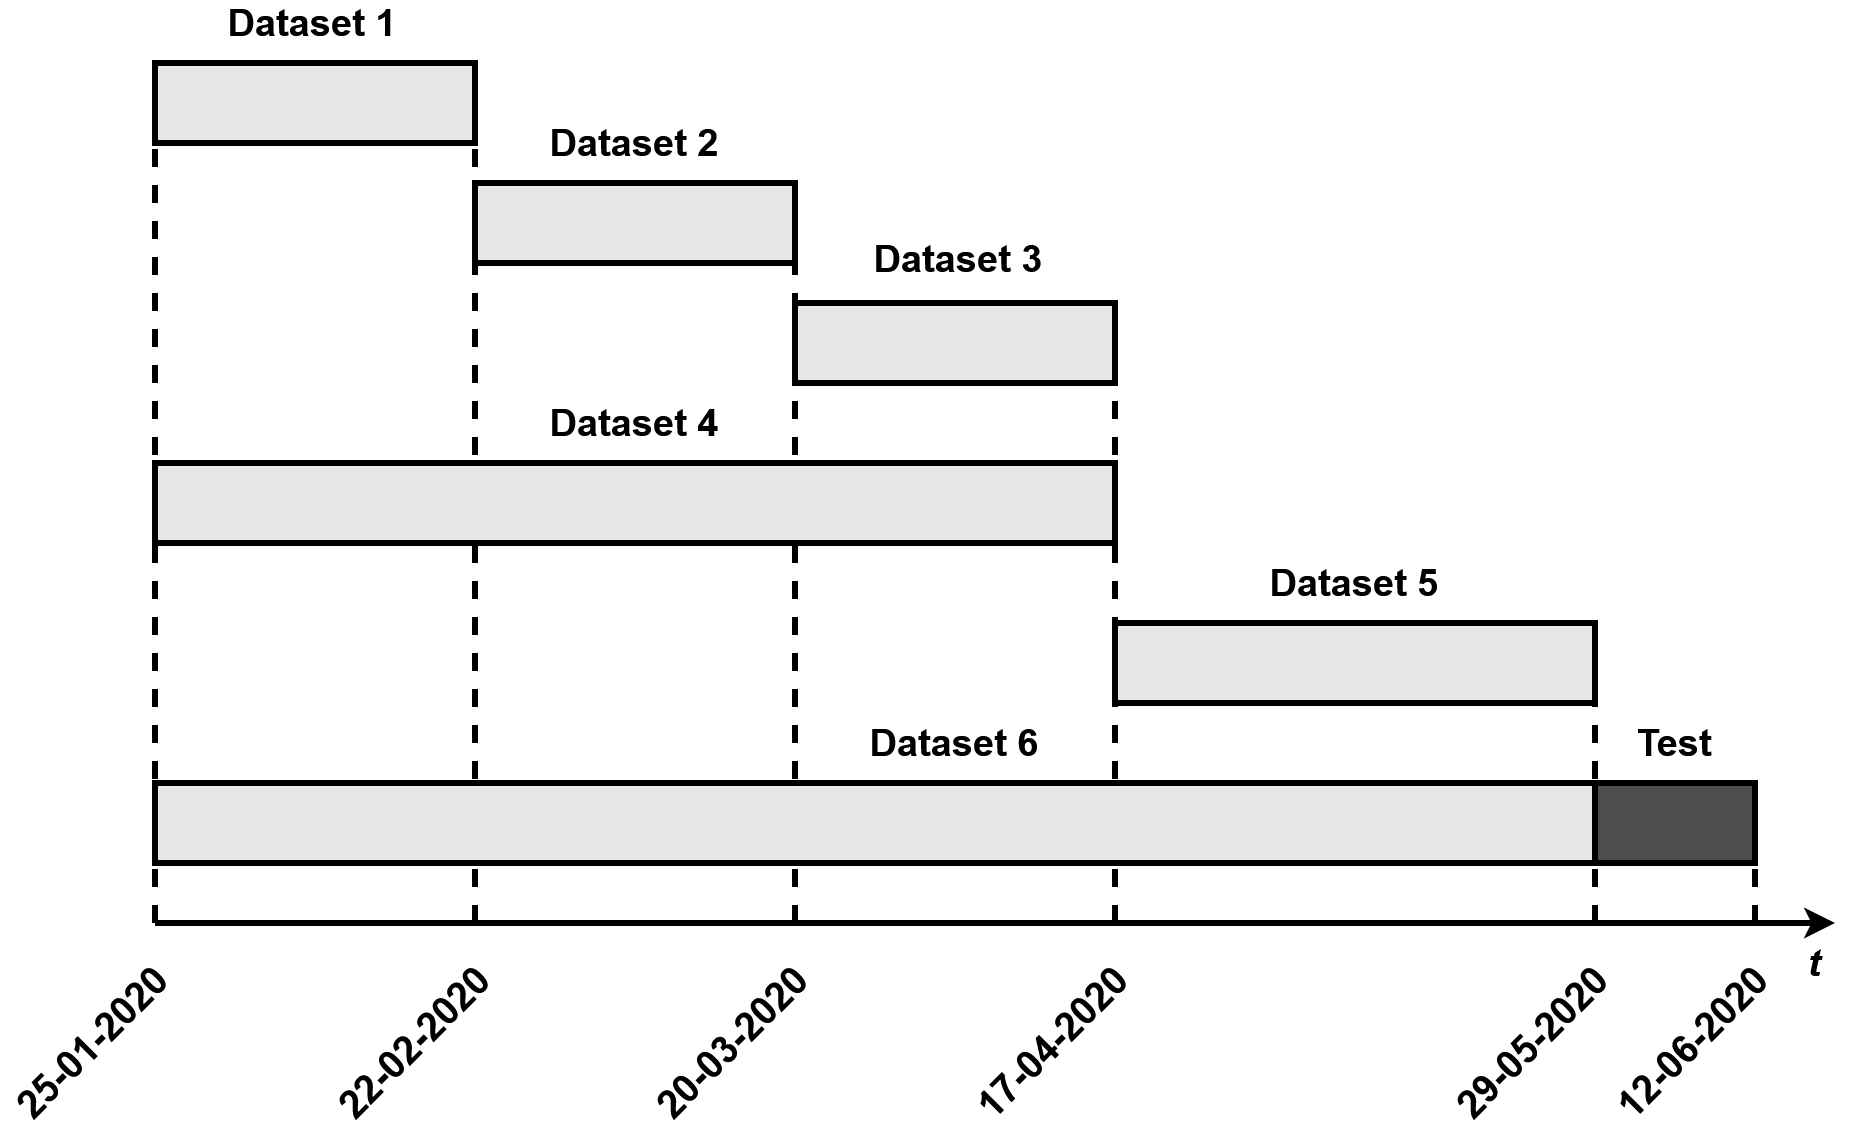
\includegraphics[width=1\textwidth]{Images/data_partition_2.png}
    \caption{Data partition diagram.}
    \label{partition}
    \end{center}
\end{figure}
The standard approach would be to split dataset 4 in training, validation and testing, but aplying Block cross-validation to to this specific case, consists of dividing the training set in a fixed number of blocks (the number of blocks chosen was 3), and perform training and validation on these blocks.
Datesets 1, 2 and 3 feature three weeks of training and one week of validation. The performance evaluation of the models is then given by the average of the performance in each of these blocks i.e., the error of the models is given by

\begin{equation}
     Model\ error =\frac {1}{k}\ \sum_{i=1}^k Error_{di},
\label{err_av}
\end{equation}

where $Model\ error$ represents the final model error, and $Error_{di}$ represents the error that the model presented while performing in dataset $i$, and $k$ represents the number of datasets used.
In this specific case, the validation error for each model is given by

\begin{equation}
     Model\ error =\frac {1}{3}\ (Error_{d1} + Error_{d2} + Error_{d3}).
\label{err_av}
\end{equation}

The great advantage of using this method is the reduction of the influence of random errors in the selection of the best model. In other words, by performing an average of 3 different sets, the robustness of the choice process is increased since different scenarios are considered and the best model is the one that performs well on average for all of them.

In a second phase, the models with the best results in the validation data set will be trained again throughout dataset 4 and tested in dataset 5. The predictions resulting from the best models in this test phase (dataset 5), will be used as input for a \ac{DenseNet}, where they will be used as training and validation data. This way, a stacked ensemble model is then constructed, which uses data resulting from the forecasts of all the finalist models to produce a final forecast. This model will then be trained throughout dataset 5 and tested on the test dataset, where its performance will be compared with the individual performance of the finalist models, trained on dataset 4 and tested also on the test dataset. Finally, the dataset 6, represents the entire dataset and presents 18 weeks.

\section{Performance evaluation metrics}\label{chap5:evaluation}

In the previous section, important details concerning the data used in this thesis were explained. One defined $Model\ error$, but did not specify which concrete metrics were used in this work. To compare the performance of the different models in the defined dataset, it is necessary to use some measures of forecast performance. In this sense, during this thesis four different measures were used that relate the real values present in the time series represented by $y_t$, and the forecast values, which are represented by $f_t$. Thus, the forecast error is given by $e_t=y_t-f_t$. The three measures presented are quite common in the literature \cite{} and are described below.

\subsection{Mean Absolute Error (MAE)}

The \ac{MAE}, is defined as

\begin{equation}
     MAE =\frac {\sum_{t=1}^n|e_t|}{n}.
\label{mae}
\end{equation}

The \ac{MAE} is known as a scale-dependent accuracy measure and measures the average absolute deviation between the forecasted values and the real ones. As a scale-dependent measure, it cannot be used to compare series series using different scales.


\subsection{Mean Squared Error (MSE) and Root Mean Squared Error (RMSE)}

The \ac{MSE}, is defined as

\begin{equation}
     MSE =\frac {1}{n}\sum_{t=1}^ne_t^2.
\label{mse}
\end{equation}

The \ac{MSE} is also known as a scale-dependent accuracy measure and measures the average squared deviation between the forecasted values and the real ones. The application of this measure is quite relevant because it doesn't allow the negative errors to cancel the positive errors and vice-versa. 

By applying the square root to the \ac{MSE}, the \ac{RMSE} is then defined as

\begin{equation}
     RMSE =\sqrt{MSE} = \sqrt{\frac {1}{n}\sum_{t=1}^ne_t^2}.
\label{rmse}
\end{equation}
Mathematically, the \ac{RMSE} is the square root of the average of the squared difference between the predicted values and the observed ones. The advantage of \ac{RMSE} over \ac{MSE} is that it is on the same scale as the targets, facilitating its interpretation in the concrete context of the problem. 

\ac{RMSE} and \ac{MAE} were the metrics implemented in the development of this research. These two measurements present some similarities, but also some differences that make it relevant to use the two metrics separately. In terms of similarities, both are expressed in the units of the variable in question, which means that both errors are easily interpretable given the context of the problem. The major difference between the two metrics lies in the contribution that individual error values make to the final result. In the case of \ac{MAE}, the contribution of individual errors follows a linear behavior. An error of 20 units contributes twice as much as an error of 10 units, and an error of 500 units contributes half as much as an error of 1000 units. In the case of \ac{RMSE} the errors are squared before being averaged, which means that this metric gives more weight to larger errors.  This means that very small errors tend to be ignored while large errors tend to be magnified. One can then conclude that \ac{RMSE} is especially useful when one intends to emphasize large errors and reduce the importance of smaller errors. It was then chosen to use both \ac{RMSE} and \ac{MAE} in the evaluation of the implemented models since both express interesting results that could be advantageous in the development of the research.


\section{Conclusion}

In this chapter, we have delved into the whole process of implementing the work of this thesis. Initially, in the section \ref{chap5:enviromnet}, we describe the different implementation environments used, and then, in the section \ref{chap5:dataset}, we describe the datset used and all the data processing that was performed. Finally, in the section \ref{chap5:evaluation}, we describe the metrics used to choose the best models designed. In the next chapter we will dive into the experimental process carried out, from the training phase of the 8 initial architectures, until the construction of the final implemented system.